\section{Auditing the evaluation set without EEG}
\label{sec:audit}

\paragraph{The stimulus order is clustered by category.}
In the released trial order, 19.7\% of consecutive trials share a category. If the same category
frequencies were in random order, 2.95\% would. The excess decays with distance but persists: 14.2\%
at lag 2, 8.9\% at lag 5, 6.7\% at lag 10 and 5.2\% at lag 50 (Figure~\ref{fig:order}). Restricting
to pairs within the same run changes these by at most 0.6 points. Runs are also unevenly composed:
a run contains a median of 30 of the 39 categories, and its most frequent category makes up a median
12.9\% of its trials (maximum 33.6\%). The trial's position within its run carries no category
information: predicting the most common training category at the same position across runs scores
3.7\%, below the majority-class rate.

\begin{figure}[t]
  \centering
  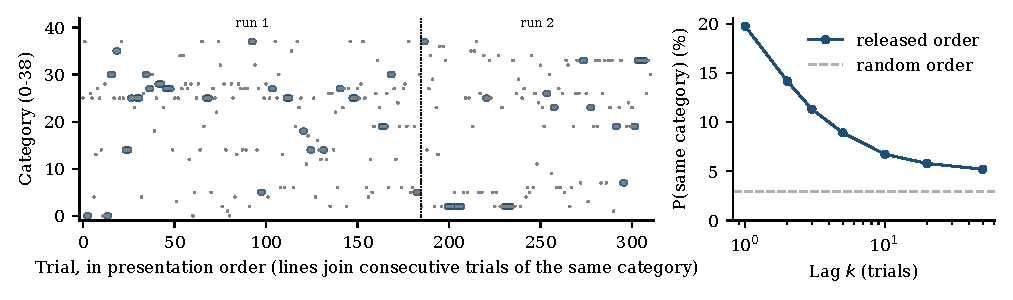
\includegraphics[width=\linewidth]{figures/fig_order.pdf}
  \caption{\textbf{Category order in the released S1 recording.} Left: category of each trial in
  runs 1--3, in presentation order (white lines separate runs). Right: probability that two trials
  $k$ positions apart share a category, against the value expected if the same categories were
  presented in random order (dashed). Source: \texttt{results/label\_baselines.json}.}
  \label{fig:order}
\end{figure}

\paragraph{Classifiers that never see EEG.}
On the released split, every evaluation trial sits between two training trials. We evaluate
classifiers that use only the training labels and each evaluation trial's position in the recording
(Table~\ref{tab:noeeg}). Copying the label of the nearest earlier training trial scores
\textbf{18.82\%} (95\% CI 16.49--21.57) on the published evaluation set, above the 13.88\% the paper
reports with EEG. A five-nearest-neighbour vote over trial position scores 20.90\%, and knowing only
which run a trial came from (predicting that run's most common training category) scores 14.41\%.
These classifiers are fitted on training labels only; none of them reads an evaluation label.

Two order controls locate the information. Shuffling all labels across the recording (1{,}000
permutations) drops the copy-previous classifier to 2.92\% on average (maximum 4.24\%). Shuffling
labels only within each run, which keeps each run's category mix but destroys the order inside it,
drops it to 5.96\% (maximum 8.25\%). Most of the 18.8\% therefore comes from adjacency within runs,
and a smaller part from run composition.

When whole runs are held out, the neighbouring training trial belongs to a different run and these
classifiers lose their advantage: copy-previous scores 2.42--5.67\% across the five run folds, and
the five-nearest vote 3.05--8.58\%.

\begin{table}[t]
\centering
\small
\caption{\textbf{Classifiers that never see EEG}, scored on the evaluation trials of each split (accuracy, \%). Each uses only training labels and the trial's position in the recording. Interleaved is the released split. Grouped splits: mean over the five folds, with the range in brackets. Uniform chance is 2.56\%. Source: \texttt{results/label\_baselines.json}.}
\label{tab:noeeg}
\setlength{\tabcolsep}{4pt}
\begin{tabular}{lcccc}
\toprule
Classifier & Interleaved & Random trial & Run holdout & Session holdout \\
\midrule
Majority class & 4.72 & 4.56 & 3.46 [2.64, 4.60] & 1.91 [0.59, 3.65] \\
Previous training trial & 18.82 & 18.57 & 4.28 [2.42, 5.67] & 3.40 [0.20, 6.84] \\
Next training trial & 20.42 & 18.57 & 5.47 [3.62, 7.69] & 3.67 [0.20, 7.62] \\
5 nearest training trials & 20.90 & 21.70 & 5.97 [3.05, 8.58] & 3.28 [0.20, 5.90] \\
Majority within run & 14.41 & 14.01 & 3.46 [2.64, 4.60] & 1.91 [0.59, 3.65] \\
Majority at run position & 3.68 & 3.52 & 3.48 [3.21, 3.77] & 3.09 [2.57, 3.79] \\
\bottomrule
\end{tabular}
\end{table}


\paragraph{EEG carries a recording-time signature.}
An EEG model can only use the order structure if the signal tells it when a trial was recorded.
We test this with deliberately content-poor features: the mean and log-variance of each channel over
the 3.3\,s epoch (244 numbers per trial, no waveform), fed to a multinomial logistic regression.
On the released split, these features identify which of the 45 runs a held-out trial came from with
\textbf{98.8\%} accuracy (chance 2.2\%). Trained to predict category instead, the same model scores
\textbf{9.05\%} on the published evaluation set (permuted-label null: mean 3.11\%, maximum 3.84\% over
five permutations) and 7.37\% on a random-trial split, but 3.55\% under run holdout (null 2.76\%,
maximum 3.77\%) and 3.08\% under session holdout (null 2.79\%). Per-trial summary statistics are
enough to recover two-thirds of the published accuracy, and only when evaluation trials have
training neighbours from the same run.
